\subsection{Average Rate of Change}
\begin{definition}[Average Rate of Change]
	The slope of the line connecting two points on a curve, known as the \textit{secant line}.
	$$Average \, Rate \, of \, Change \, = \frac{f(b) - f(a)}{b - a}$$
\end{definition}

\begin{example}[Graph] 
	\hfill
	\begin{center}
	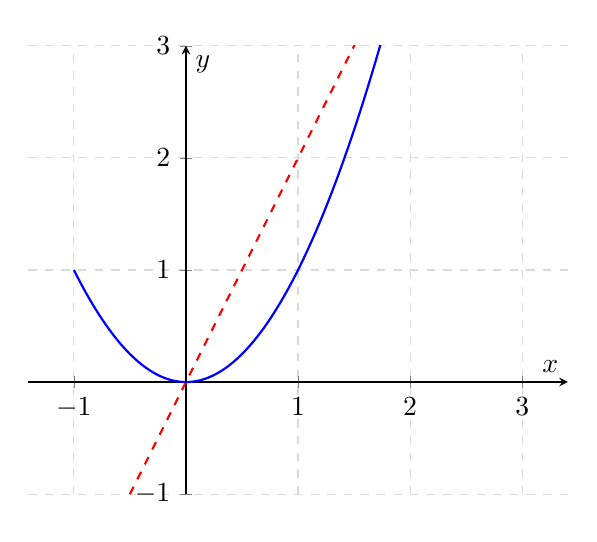
\begin{tikzpicture}
		\begin{axis}[
		    axis lines = center,
		    xlabel = $x$,
		    ylabel = $y$,
		    xmin = -1, xmax = 3,
		    ymin = -1, ymax = 3,
		    grid = both,
		    grid style = {dashed, gray!30},
		    axis equal
		]
		    \addplot [domain=-1:2.5, samples=100, thick, blue] {x^2};
		    \addplot [domain=-0.5:2.5, samples=2, dashed, red, thick] {2*x};
		\end{axis}
	\end{tikzpicture}
	\end{center}
	$$a = 0, b = 2$$
	$$\frac{f(2) - f(0)}{2 - 0} = \frac{4 - 0}{2 - 0} = 2$$
\end{example}

\begin{example}[Algebraic]
	$$f(x) = x^2 - 2x \, Find \, average \, rate \, of \, change$$
	$$From \, x = 3 \, to \, x = 5$$
	$$f(3) = (3)^2 - 2(3)$$
	$$f(3) = 3$$
	$$f(5) = (5)^2 - 2(5)$$
	$$f(5) = 15$$
	$$(3, 3) \, (5, 15)$$
	$$Average \, Rate \, of \, Change \, = \frac{15 - 3}{5 - 3}$$
	$$Average \, Rate \, of \, Change \, = \frac{12}{2} \to 6$$
\end{example}
